%%% DOCUMENTCLASS 
%%%-------------------------------------------------------------------------------

\documentclass[
a4paper, % Stock and paper size.
11pt, % Type size.
% article,
% oneside, 
onecolumn, % Only one column of text on a page.
% openright, % Each chapter will start on a recto page.devguide
% openleft, % Each chapter will start on a verso page.
openany, % A chapter may start on either a recto or verso page.
]{memoir}

%%% PACKAGES 
%%%------------------------------------------------------------------------------

\usepackage[utf8]{inputenc} % If utf8 encoding
% \usepackage[lantin1]{inputenc} % If not utf8 encoding, then this is probably the way to go
\usepackage[T1]{fontenc}    %
\usepackage{lmodern}
\usepackage[english]{babel} % English please
\usepackage[final]{microtype} % Less badboxes
\usepackage[stable]{footmisc} % Footnotes in section titles
\usepackage{url}
\usepackage{mathrsfs}

% \usepackage{kpfonts} %Font

\usepackage{amsmath,amssymb,mathtools} % Math

% \usepackage{tikz} % Figures
\usepackage{graphicx} % Include figures
\usepackage{makeidx}
\usepackage{import}
\usepackage{subcaption}
\captionsetup{compatibility=false}

%%% PAGE LAYOUT 
%%%-----------------------------------------------------------------------------
\setlrmarginsandblock{0.15\paperwidth}{*}{1} % Left and right margin
\setulmarginsandblock{0.2\paperwidth}{*}{1}  % Upper and lower margin
\checkandfixthelayout

\newlength\forceindent
\setlength{\forceindent}{\parindent}
\setlength{\parindent}{0cm}
\renewcommand{\indent}{\hspace*{\forceindent}}
\setlength{\parskip}{1em}


%%% SECTIONAL DIVISIONS
%%%------------------------------------------------------------------------------

\maxsecnumdepth{subsection} % Subsections (and higher) are numbered
\setsecnumdepth{subsection}

\makeatletter %
\makechapterstyle{standard}{
  \setlength{\beforechapskip}{0\baselineskip}
  \setlength{\midchapskip}{1\baselineskip}
  \setlength{\afterchapskip}{8\baselineskip}
  \renewcommand{\chapterheadstart}{\vspace*{\beforechapskip}}
  \renewcommand{\chapnamefont}{\centering\normalfont\Large}
  \renewcommand{\printchaptername}{\chapnamefont \@chapapp}
  \renewcommand{\chapternamenum}{\space}
  \renewcommand{\chapnumfont}{\normalfont\Large}
  \renewcommand{\printchapternum}{\chapnumfont \thechapter}
  \renewcommand{\afterchapternum}{\par\nobreak\vskip \midchapskip}
  \renewcommand{\printchapternonum}{\vspace*{\midchapskip}\vspace*{5mm}}
  \renewcommand{\chaptitlefont}{\centering\bfseries\LARGE}
%  \renewcommand{\printchaptertitle}[1]{\chaptitlefont ##1}
  \renewcommand{\afterchaptertitle}{\par\nobreak\vskip \afterchapskip}
}
\makeatother

%\chapterstyle{standard}
\chapterstyle{madsen}

\setsecheadstyle{\normalfont\large\bfseries}
\setsubsecheadstyle{\normalfont\normalsize\bfseries}
\setparaheadstyle{\normalfont\normalsize\bfseries}
\setparaindent{0pt}\setafterparaskip{0pt}

%%% FLOATS AND CAPTIONS
%%%------------------------------------------------------------------------------

\makeatletter                  % You do not need to write [htpb] all the time
\renewcommand\fps@figure{htbp} %
\renewcommand\fps@table{htbp}  %
\makeatother                   %

\captiondelim{\space } % A space between caption name and text
\captionnamefont{\small\bfseries} % Font of the caption name
\captiontitlefont{\small\normalfont} % Font of the caption text

% incompatible with subcaption package so commented out for now
%\changecaptionwidth          % Change the width of the caption
%\captionwidth{1\textwidth} %

%%% ABSTRACT
%%%------------------------------------------------------------------------------

\renewcommand{\abstractnamefont}{\normalfont\small\bfseries} % Font of abstract title
\setlength{\absleftindent}{0.1\textwidth} % Width of abstract
\setlength{\absrightindent}{\absleftindent}

%%% HEADER AND FOOTER 
%%%------------------------------------------------------------------------------

\makepagestyle{standard} % Make standard pagestyle

\makeatletter                 % Define standard pagestyle
\makeevenfoot{standard}{}{}{} %
\makeoddfoot{standard}{}{}{}  %
\makeevenhead{standard}{\bfseries\thepage\normalfont\qquad\small\leftmark}{}{}
\makeoddhead{standard}{}{}{\small\rightmark\qquad\bfseries\thepage}
% \makeheadrule{standard}{\textwidth}{\normalrulethickness}
\makeatother                  %

\makeatletter
\makepsmarks{standard}{
\createmark{chapter}{both}{shownumber}{\@chapapp\ }{ \quad }
\createmark{section}{right}{shownumber}{}{ \quad }
\createplainmark{toc}{both}{\contentsname}
\createplainmark{lof}{both}{\listfigurename}
\createplainmark{lot}{both}{\listtablename}
\createplainmark{bib}{both}{\bibname}
\createplainmark{index}{both}{\indexname}
\createplainmark{glossary}{both}{\glossaryname}
}
\makeatother                               %

\makepagestyle{chap} % Make new chapter pagestyle

\makeatletter
\makeevenfoot{chap}{}{\small\bfseries\thepage}{} % Define new chapter pagestyle
\makeoddfoot{chap}{}{\small\bfseries\thepage}{}  %
\makeevenhead{chap}{}{}{}   %
\makeoddhead{chap}{}{}{}    %
% \makeheadrule{chap}{\textwidth}{\normalrulethickness}
\makeatother

\nouppercaseheads
\pagestyle{standard}               % Choosing pagestyle and chapter pagestyle
\aliaspagestyle{chapter}{chap} %

%%% NEW COMMANDS
%%%-----------------------------------------------------------------------------

%%% Nektar++ version and Tutorial Root
\endlinechar=-1\relax
\newread\filever
\openin\filever=VERSION
\read\filever to\linever
\newcommand{\nekver}{\linever}
\closein\filever

% relurl takes filename as first arg and url suffix (less filename) as second.
\ifdefined\HCode
\newcommand{\relurl}[2]{\href{#1}{\underline{#1}}}
\else
\newcommand{\relurl}[2]{\url{http://doc.nektar.info/tutorials/\nekver/#2/#1}}
\fi
\endlinechar=13\relax

\newcommand{\p}{\partial} %Partial
% Or what ever you want


%%% CODE SNIPPETS, COMMANDS, ETC
%%%-----------------------------------------------------------------------------
\usepackage{xcolor}
\usepackage{listings} % Display code / shell commands
\usepackage{lstautogobble}
\usepackage{xspace}
\usepackage{xcolor}
\usepackage{listings} % Display code / shell commands
\usepackage{lstautogobble}
%\newcommand{\shellcommand}[1]{\begin{lstlisting} \#1 \end{lstlisting}
\lstset{
  breaklines=true
}
\lstdefinestyle{BashInputStyle}{
  language=bash,
  basicstyle=\small\ttfamily,
%  numbers=left,
%  numberstyle=\tiny,
%  numbersep=3pt,
  frame=single,
  columns=fullflexible,
  backgroundcolor=\color{yellow!10},
  linewidth=0.95\linewidth,
  xleftmargin=0.05\linewidth,
  keepspaces=true,
  breaklines=true,
  framesep=5pt,
  rulecolor=\color{black!30},
  aboveskip=10pt,
  autogobble=true
}
\definecolor{gray}{rgb}{0.4,0.4,0.4}
\definecolor{darkblue}{rgb}{0.0,0.0,0.6}
\definecolor{darkred}{rgb}{0.6,0.0,0.0}
\definecolor{cyan}{rgb}{0.0,0.6,0.6}
\definecolor{maroon}{rgb}{0.5,0.0,0.0}
\lstdefinelanguage{XML}
{
  basicstyle=\ttfamily\footnotesize,
  morestring=[b]",
  moredelim=[s][\bfseries\color{maroon}]{<}{\ },
  moredelim=[s][\bfseries\color{maroon}]{</}{>},
  moredelim=[l][\bfseries\color{maroon}]{/>},
  moredelim=[l][\bfseries\color{maroon}]{>},
  morecomment=[s]{<?}{?>},
  morecomment=[s]{<!--}{-->},
  commentstyle=\color{gray},
  stringstyle=\color{orange},
  identifierstyle=\color{darkblue},
  breaklines=true
}
\lstdefinestyle{XMLStyle}{
  language=XML,
  basicstyle=\sffamily\footnotesize,
  numbers=left,
  numberstyle=\tiny,
  numbersep=3pt,
  frame=,
  columns=fullflexible,
  backgroundcolor=\color{black!05},
  linewidth=0.95\linewidth,
  xleftmargin=0.05\linewidth,
  breaklines=true
}
\lstdefinestyle{C++Style}{
  language=C++,
  basicstyle=\ttfamily\footnotesize,
  numbers=left,
  numberstyle=\tiny,
  numbersep=3pt,
  frame=,
  columns=fullflexible,
  backgroundcolor=\color{black!05},
  linewidth=0.95\linewidth,
  xleftmargin=0.1\linewidth,
  showspaces=false,
  showstringspaces=false,
  breaklines=true,
  keywordstyle=\color{blue}\ttfamily,
  stringstyle=\color{red}\ttfamily,
  commentstyle=\color{violet}\ttfamily,
  morecomment=[l][\color{teal}]{\#}
}

\ifdefined\HCode
\newcommand{\inltt}[1]{\texttt{#1}}
\newcommand{\inlsh}[1]{\texttt{#1}}
\else
\newcommand{\inltt}[1]{\tikz[anchor=base,baseline]\node[inner sep=3pt,
rounded corners,outer sep=0,draw=black!30,fill=black!05]{\small\texttt{#1}};}
\newcommand{\inlsh}[1]{\tikz[anchor=base,baseline]\node[inner sep=2pt,
outer sep=0,fill=black!05]{\texttt{#1}};}
\fi
\newcommand{\nekpp}{{\em Nektar++}\xspace}

% Highlight box
\usepackage{environ}
\usepackage[tikz]{bclogo}
\usetikzlibrary{calc}

% Only use fancy boxes for PDF
\ifdefined\HCode
\NewEnviron{notebox}{\textbf{Note:} \BODY}
\NewEnviron{warningbox}{\textbf{Warning:} \BODY}
\NewEnviron{tipbox}{\textbf{Tip:} \BODY}
\NewEnviron{custombox}[3]{\textbf{#1} \BODY}
\else
\NewEnviron{notebox}
  {\par\medskip\noindent
  \begin{tikzpicture}
    \node[inner sep=5pt,fill=black!10,draw=black!30] (box)
    {\parbox[t]{.99\linewidth}{%
      \begin{minipage}{.1\linewidth}
      \centering\tikz[scale=1]\node[scale=1.5]{\bcinfo};
      \end{minipage}%
      \begin{minipage}{.9\linewidth}
      \textbf{Note}\par\smallskip
      \BODY
      \end{minipage}\hfill}%
    };
   \end{tikzpicture}\par\medskip%
}
\NewEnviron{warningbox}
  {\par\medskip\noindent
  \begin{tikzpicture}
    \node[inner sep=5pt,fill=red!10,draw=black!30] (box)
    {\parbox[t]{.99\linewidth}{%
      \begin{minipage}{.1\linewidth}
      \centering\tikz[scale=1]\node[scale=1.5]{\bcdanger};
      \end{minipage}%
      \begin{minipage}{.9\linewidth}
      \textbf{Warning}\par\smallskip
      \BODY
      \end{minipage}\hfill}%
    };
   \end{tikzpicture}\par\medskip%
}
\NewEnviron{tipbox}
  {\par\medskip\noindent
  \begin{tikzpicture}
    \node[inner sep=5pt,fill=green!10,draw=black!30] (box)
    {\parbox[t]{.99\linewidth}{%
      \begin{minipage}{.1\linewidth}
      \centering\tikz[scale=1]\node[scale=1.5]{\bclampe};
      \end{minipage}%
      \begin{minipage}{.9\linewidth}
      \textbf{Tip}\par\smallskip
      \BODY
      \end{minipage}\hfill}%
    };
   \end{tikzpicture}\par\medskip%
}
\NewEnviron{custombox}[3]
  {\par\medskip\noindent
  \begin{tikzpicture}
    \node[inner sep=5pt,fill=#3!10,draw=black!30] (box)
    {\parbox[t]{.99\linewidth}{%
      \begin{minipage}{.1\linewidth}
      \centering\tikz[scale=1]\node[scale=1.5]{#2};
      \end{minipage}%
      \begin{minipage}{.9\linewidth}
      \textbf{#1}\par\smallskip
      \BODY
      \end{minipage}\hfill}%
    };
   \end{tikzpicture}\par\medskip%
}
\fi

%%% TABLE OF CONTENTS AND INDEX
%%%-----------------------------------------------------------------------------

\maxtocdepth{subsection} % Only parts, chapters and sections in the table of contents
\settocdepth{subsection}

\makeindex

%\AtEndDocument{\addtocontents{toc}{\par}} % Add a \par to the end of the TOC

%%% INTERNAL HYPERLINKS
%%%-----------------------------------------------------------------------------
\usepackage[linktoc=all,hyperfootnotes=false]{hyperref}   % Internal hyperlinks
\hypersetup{
colorlinks,
citecolor=darkblue,
filecolor=darkblue,
linkcolor=darkblue,
urlcolor=darkblue,
pdfborder={0 0 0},      % No borders around internal hyperlinks
}
\usepackage{memhfixc}   %


%%% PRETTY TITLE PAGE FOR PDF DOC
%%%-----------------------------------------------------------------------------
\ifdefined\HCode
\else
\makeatletter
\newlength\drop
\newcommand{\br}{\hfill\break}
\newcommand*{\titlepage}{%
    \thispagestyle{empty}
    \begingroup% Gentle Madness
    \drop = 0.1\textheight
    \vspace*{\baselineskip}
    \vfill
    \hbox{%
      \hspace*{0.1\textwidth}%
      \rule{1pt}{\dimexpr\textheight-28pt\relax}%
      \hspace*{0.05\textwidth}% 
      \parbox[b]{0.85\textwidth}{%
        \vbox{%
          {
\includegraphics[width=0.2\textwidth]{img/icon-blue.png}\par}
          \vskip1.00\baselineskip
          {\Huge\bfseries\raggedright\@title\par}
          \vskip2.37\baselineskip
          %{\huge\bfseries Version \input{../../VERSION}\par}
 %         \vskip4\baselineskip
          {\huge\bfseries \textcolor{darkred}{Developer's Guide}\par}
          \vskip1.0\baselineskip
          {\large\bfseries Editors: Robert M. (Mike) Kirby, Spencer J. Sherwin, Chris D. Cantwell and David Moxey \par}
          \vskip1.0\baselineskip
          {\large\bfseries \textcolor{darkblue}{A distributed working draft for further contribution by the Nektar++ community} \par}
          \vskip1.0\baselineskip
          {\large\bfseries\@date\par}
          \vspace{0.3\textheight}
          {\small\noindent\@author}\\[\baselineskip]
        }% end of vbox
      }% end of parbox
    }% end of hbox
    \vfill
    \null
\endgroup}
\makeatother
\fi

\definecolor{LightGrey}{rgb}{0.9,0.9,0.9}
\newcounter{taskcount}[chapter]
\newcommand\gmsh{\emph{Gmsh}~}
\newcommand\paraview{\emph{Paraview}~}
\newcommand\nektar{\emph{Nektar++}\xspace}
\newcommand\devguidepath{\texttt{/nektutorial}}
\ifdefined\HCode
\NewEnviron{devguidetask}{
\addtocounter{taskcount}{1}
\textbf{Task: \arabic{chapter}.\arabic{taskcount}} \BODY
}
\else
\NewEnviron{devguidetask}
  {\addtocounter{taskcount}{1}
  \par\medskip\noindent
  \begin{tikzpicture}
    \node[inner sep=5pt,fill=black!10,draw=black!30] (box)
    {\parbox[t]{.99\linewidth}{%
      \begin{minipage}[t]{.1\linewidth}
      \vspace{-5mm}
      \centering\tikz[scale=1]\node[scale=1.5]{\bccrayon};
      \end{minipage}%
      \begin{minipage}[t]{.9\linewidth}
      \textbf{{Task \arabic{chapter}.\arabic{taskcount}}}\par\smallskip
      \BODY
      \end{minipage}\hfill}%
    };
   \end{tikzpicture}\par\medskip%
}
\fi
\ifdefined\HCode
\NewEnviron{advanceddevguidetask}{
\addtocounter{taskcount}{1}
\textbf{Advanced Task: \arabic{chapter}.\arabic{taskcount}} \BODY
}
\else
\NewEnviron{advanceddevguidetask}
  {\addtocounter{taskcount}{1}
  \par\medskip\noindent
  \begin{tikzpicture}
    \node[inner sep=5pt,fill=black!10,draw=black!30] (box)
    {\parbox[t]{.99\linewidth}{%
      \begin{minipage}[t]{.1\linewidth}
      \vspace{-5mm}
      \centering\tikz[scale=1]\node[scale=1.5]{\bccrayon};
      \end{minipage}%
      \begin{minipage}[t]{.9\linewidth}
      \textbf{{Advanced Task \arabic{chapter}.\arabic{taskcount}}}\par\smallskip
      \BODY
      \end{minipage}\hfill}%
    };
   \end{tikzpicture}\par\medskip%
}
\fi

\newcommand\devguidecommand[1]{
    \par{\vspace{1ex}
         \addtolength{\leftskip}{2mm}\texttt{#1}\par\vspace{1ex}}
}
\newcommand\devguidenote[1]{\par{\textbf{Note: }#1}}


%%% THE DOCUMENT
%%% Where all the important stuff is included!
%%%-------------------------------------------------------------------------------

\author{Department of Aeronautics, Imperial College London, UK\newline
Scientific Computing and Imaging Institute, University of Utah, USA}
\date{\today}


\DeclareOldFontCommand{\bf}{\normalfont\bfseries}{\mathbf}

\usepackage{makeidx}
\usepackage{hyperref}
\hypersetup{
    colorlinks=true,
    linkcolor=blue,
    filecolor=magenta,      
    urlcolor=cyan,
}
 
\urlstyle{same}
 
 \makeindex

\newcommand\nek{\emph{Nektar++}}
\newcommand\shp{spectral/$hp$}
\newcommand\Shp{Spectral/$hp$}
\newcommand{\GIT}{\textit{git}}
\def\code#1{\texttt{#1}}
\newcommand\hlink{\hyperlink}
\newcommand\htarget{\hypertarget}%%%
\newcommand{\BM}[1]{\mbox{\boldmath $#1$}}
\newcommand{\BMB}[1]{\mbox{$\mathbb #1$}}

%Yu Pan's commands
\usepackage{tikz}
\usetikzlibrary{positioning}
\usetikzlibrary{calc}
% \usepackage{multicol}
% \setlength{\columnsep}{0.5cm}
\tikzset{abs1/.style={xshift=3cm,yshift=2cm}}
\usetikzlibrary{shapes.geometric,arrows,automata}
\tikzstyle{arrow}=
[thick,->,>=stealth]
\tikzstyle{arrow1}=
[thick,dashed,->,>=stealth]

\usepackage{standalone}
\usepackage{rotating}
%end of Yu Pan's commands

\title{A Programmer's Guide to Nektar++}

%\makeatletter\@addtoreset{chapter}{part}\makeatother%
\begin{document}

%\frontmatter

% Render pretty title page if not building HTML
\ifdefined\HCode
\begin{center}
    
\includegraphics[width=0.1\textwidth]{img/icon-blue.png}
\end{center}
\maketitle
\begin{center}
       \huge{Nektar++ Developer's Guide}
\end{center}
\else
\titlepage
\fi

%\clearpage

%\ifx\HCode\undefined
%\tableofcontents*
%\fi
%
%\clearpage

%\input{test.tex}

\tableofcontents

\import{preface/}{preface}

% Introduction
\chapter{Introduction}

\nek{} \cite{CantwellMCBRMGYLEJXMENVBKS2015}, is an open-source software framework designed to support the development of 
high-performance scalable solvers for partial differential equations using the spectral/{\em hp\/} element method.   
What in part makes \nek{} unique is that it is  
an initiative to overcome the mathematical complexities of the methods by encapsulating them within an efficient cross-platform C++ software environment, consequently making the techniques more accessible to the broader scientific and industrial communities. The software supports a variety of discretization techniques and 
implementation strategies \cite{VosSK2010,CantwellSKK2011a,CantwellSKK2011b,BolisCKS2014},
supporting methods research as well as application-focused computation, and the multi-layered structure of the framework allows the user to embrace as much or as little of the complexity as they need. The libraries capture the mathematical constructs of spectral/{\em hp\/} element methods in the form of a hierarchy of C++ components, while the associated collection of pre-written PDE solvers provides out-of-the-box functionality across a range of application areas, as well as a template for users who wish to develop solutions for addressing questions in their own scientific domains.

% Overview of Nektar++ and its goals/features
The cross-platform nature of the software libraries enables the rapid development of solvers for use in a wide variety of computing environments. The code accommodates both small research problems, suitable for desktop computers, and large-scale industrial simulations, requiring modern HPC infrastructure, where there is a need to maintain efficiency and scalability up to many thousands of processor cores.

\nek{} provides a single codebase with the following key features:
\begin{itemize}
  \item Arbitrary-order \shp{} element discretisations in one, two and three
  dimensions;
  \item Support for variable polynomial order in space and heterogeneous
  polynomial order within two- and three-dimensional elements;
  \item High-order representation of the geometry;
  \item Continuous Galerkin, discontinuous Galerkin and hybridised discontinuous
  Galerkin projections;
  \item Support for a Fourier extension of the spectral element mesh;
  \item Support for a range of linear solvers and preconditioners;
  \item Multiple implementation strategies for achieving linear algebra
  performance on a range of platforms;
  \item Efficient parallel communication using MPI showing strong scaling up to
  8192-cores on Archer, the UK national HPC system;
  \item A range of time integration schemes implemented using generalised linear
  methods; and
  \item Cross-platform support for Linux, OS X and Windows operating
  systems.
\end{itemize}

In addition to the core functionality listed above, \nek{} includes a
number of solvers covering a range of application areas. A range
of pre-processing and post-processing utilities are also included with support
for popular mesh and visualization formats, and an extensive test suite ensures
the robustness of the core functionality.


%%%%%%%%%%%%%%%%%%%%%%%%%%%%%%%%%%%%%%%%%%%%%%%%%%

\section{The {\em Ethos} of Nektar++}


As with any research effort, one is required to decide on a set of guiding principles that will 
drive the investigation.  Similarly with a software development effort of this form, we  
spent considerable time early on considering which aspects we wanted to be distinctive about {\nek} and also
what guiding principles would be most suitable to support both the goals and the boundaries of what
we wanted to do.  We did this for at least two reasons:  (1) We acknowledged then and now that
there are various software packages and open-source efforts that deal with finite element frameworks,
and so we wanted to be able to understand and express to people those things we thought were
distinctive to us -- that is, our ``selling points''.  (2) We also acknowledged, from our own experience
on software projects, that if we did not set up some collection of guiding principles for our work, that
we would gravitate towards trying to be ``all things to all men", and in doing so be at odds with the
first item.  Below are a list of the guiding principles, the ``ethos'', of the Nektar++ software development
effort.

\paragraph{Principles:}
The following are our three guiding principles for {\nek} which respect (1) above:

\begin{itemize}
\item \textbf{Efficiently:} {\nek} was to be a ``true'' high-order code.  ``True'' is put in quotations because we acknowledge
that high-order means different things to different communities.  Based upon a review of the literature, we 
came to the conclusion that part of our {\em h-to-p} philosophy should be that we accommodate polynomial
degrees ranging from zero (finite volumes) or one (traditional linear finite elements) up to what is considered
``spectral'' (pseudospectral) orders of 16$^{th}$ degree.  As part of our early work \cite{VosSK2010}, we established that in
order to span this range of polynomial degrees and attempt to maintain some level of computational 
efficiency, we would need to develop {\em order-aware} algorithms:  that is, we would need to utilize
different (equivalent) algorithms appropriate for a particular order.  This principle was the starting point
of our {\em h-to-p efficiently} branding and continues to be a driving principle of our work. 

\item \textbf{Transparently:} {\nek} was to be agnostic as to what the ``right'' way to discretize a partial differential equation (PDE).
``Right'' is put in quotations to acknowledge that like the issue of polynomial order, there appear to be different
``camps'' who hold very strong views as to which discretization method should be used.   Some might concede that
continuous Galerkin methods are very natural for elliptic and parabolic PDEs and then work very laboriously to 
shoehorn all mixed-type PDEs (such as the incompressible Navier-Stokes equations) into this form.  This holds
true (similarly) for finite volume and dG proponents with regards to hyperbolic problems (and those systems that are
dominated by hyperbolicity).  Our goal was to be a high-order finite element framework that allowed users to experiment with
continuous Galerkin (cG) and discontinuous Galerkin (dG) methods.  After our original developments, we incorporated 
Flux-Reconstruction Methods (FR Methods) into our framework; this confirmed that generality of our approach as our
underlying library components merely needed new features added to accommodate the FR perspective on dG methods.
As stated earlier, this is in part why we use the term \shp{} as it allows us to capture all these various methods (e.g., cG, dG and FR)
under one common element-and-order terminology.

\item \textbf{Seamlessly:}  {\nek} was to be a code that could run from the desktop (or laptop) to exascale, seamlessly.  It was our
observation that many {\em grand challenge} efforts target petascale and exascale computing, with the idea that in the future
what is done now on a supercomputer will be done on the desktop.  The supercomputer of today is in a rack within five
years and on our desktop in ten years.  However, we also acknowledged that many of our end users were interested in computing
{\em now}.  That is, following from their engineering tradition they had an engineering or science problem to solve, and they wanted 
the ability to run on machines ranging from their laptops to exascale as the problem demanded.  Not all problems fit on your laptop, 
and yet not all problems are exascale problems.  Like with our {\em h-to-p efficiently} approach, we wanted our algorithms and code
development to allow a range of choices in the hands of the engineer.
\end{itemize}

Based upon these principles, our long-term vision is a software framework that allows the engineer the flexibility to make all
these critical choices (elemental discretization, polynomial order, discretization methodology, algorithms to employ, and 
architecture-specific details) while at the same time having {\em smart and adaptive defaults}.  That is, we want to 
accommodate both the engineer that wants control over all the various knobs that must be set to actualize a simulation run
and the engineer that wants to remain at the high-level and let the software system choose what is best in terms of discretization,
polynomial order, algorithm choice, etc.  We want the flexibility to self tune, while targeting auto-tuning.

The three items above denote the principles of our development efforts.  We now present the ``guardrails''.  By guardrails, we mean
the guidelines we use to help steer us along towards our goal as stated above.  These are not meant to be absolutes necessarily,
but are considerations we often use to try to keep us on track in terms of respecting our three guiding principles above.

\paragraph{Guardrails:}

\begin{itemize}
\item We are principally concerned with advection-reaction-diffusion and conservation law problems.   There are many
simulation codes that are deal with solid mechanics, and we did not see ourselves as being a competitor with them.  As such,
we did not initially construct our framework to inherently deal with $H-div$ and $H-curl$ spaces (and their respective element types).
Our perspective was to hold a system of scalar fields and, as needed, constrain them to respect certain mathematical properties.  

\item We rely heavily on the ability to do tensor-product-based quadrature.  Although our more recent additions to the Point and Basis
information within our library allows for unstructured quadrature, many of our algorithms are designed to try to capitalize on
tensor-product properties.

\item As we said earlier, we have designed our code to run at a range of orders, from one to sixteen.  However, we acknowledge that 
for many simulation regimes, we often do not run at the lowest and/or the highest orders.  For many applications, the sweet spot seems
to be polynomials of degree four through eight.  At the present time, a reasonable amount of time and effort has been spent optimizing
for this range.

\item The robustness of our testing is often dictated by the application areas that have funded our code development.  At the present
time, our incompressible Navier-Stokes solver is probably the most tested of our solvers, followed by our ADR solver.  We make
every attempt to test our codes thoroughly; however we benefit greatly from various users ``stress-testing'' our codes and providing 
feedback on things we can improve (or better yet, suggesting coding solutions).
\end{itemize}


%%%%%%%%%%%%%%%%%%%%%%%%%%%%%%%%%%%%%%%%%%%%%%%%%%

\section{The Structure of Nektar++}

When we speak of {\nek}, it often means different things to different people, all under an umbrella of code.  For the founders of {\nek}, 
the view was that the core of {\nek} was the library, and that everything else was to be built around or on top of our basic \shp{} framework.
For others, the heart of {\nek} are its solvers -- the collection of simulation codes, built upon the library, that enable users to solve
science and engineering problems.   For a smaller group of people, it is all the add-ons that we provide in our utilities, from our
mesh generation techniques to our visualization software ideas.   

For the purposes of this document, we will structure our discussions into three main parts:  library functionality, solvers and utilities.  In this
section, we will provide an overview of the structure of the libraries.  We will start by giving a quick overview of the basic subdirectories
contained within {\em library} and their purpose.  We will then provide a bottom-up description of how the library can be viewed, as well
as a top-down perspective.  Each perspective (bottom-up or top-down) is fully consistent with each other; the advantage of these approaches
is that they help the future developer understand the library as someone trying to build up towards our solvers, or conversely someone trying
to understand our solver functionality having already been a solver user and now trying to understand the library components on which it was built.

The basic subdirectories with the {\em library} are as follows:

\noindent{\textbf{LibUtilities:}}  This library contains all the basic mathematical and computer science building blocks of the {\nek} code.

\noindent{\textbf{StdRegions:}} This library contains the objects that express ``standard region'' data and operations.  In one dimension, this is the StdSegment.  In two 
dimensions, this is the StdTri (Triangle) and StdQuad (Quadrilateral).  In three dimensions, this is the StdTet (Tetrahedra), 
StdHex (Hexahedra), StdPrism (Prism) and StdPyr (Pyramid).  These represent the seven different standardized reference regions over which 
we support differentiation and integration. 

\noindent{\textbf{SpatialDomains:}} This library contains the mesh and elemental geometric information.  In particular, this part of the library deals with the basic mesh 
data structures, and the mapping information (such as Jacobians) from StdRegions to LocalRegions.

\noindent{\textbf{LocalRegions:}}  This library contains objects that express data and operations on individual physical elements of the computational mesh.  Local regions are \shp{} elements in
world-space (either straight-/planar-sided or curved-sided).  Using C++ terminology, a local region object {\em is-a} standard region object and {\em has-a} spatial domain object.

\noindent{\textbf{MultiRegions:}} This library holds the data structures that represent sets of elements (local regions).  At the most fundamental 
level, these represent the union of local regions into a (geometrically-contiguous) space.  By specifying the interaction of these elements, the function space they represent and/or the approximation method is defined.  It is at this point in the hierarchy that a set of (local region) elements can be thought of as representing a dG or cG field.

\noindent{\textbf{Collections:}} In this library we amalgamate, in a linear algebra sense, the action of key operators on multiple 
(standard region or local region) elements into a single, memory-efficient block. These strategies depend on external
factors such as BLAS implementation and the geometry of interest. 

\noindent{\textbf{GlobalMapping:}} This library supports the analytical mapping of complex physical domains to simpler computational domains.

\noindent{\textbf{NekMeshUtils:}} This library contains processing modules for the generation (potentially from CAD geometries), conversion and manipulation of high-order meshes.

\noindent{\textbf{SolverUtils:}} This library contains data structures and algorithms which form the basis of solvers, or provide auxiliary functionality.

\noindent{\textbf{UnitTests:}} This part of the library contains unit tests that allow us to verify the correctness of the core functionality within {\nek}.  These are useful for verifying
that new additions or modifications to the lower-levels of the code do not compromise existing functionality or correctness.

%%%%%%%%%%%%%%%%%%%%%%%%%%%%%%
\subsubsection{Bottom-Up Perspective}

The bottom-up perspective on the library is best understood from Figures \ref{intro:stdtolocal} -- \ref{intro:structure1}.  In Figure \ref{intro:stdtolocal}, we
take the view of understanding the geometric regions over which we build approximations.  Our starting point is within the StdRegions library, in which
we define our canonical standard regions.  There are seven fundamental regions supported by \nek{}:  segments (1D), triangles and quadrilaterals (2D) and tetrahedra, hexahedra,
prisms and pyramids (3D).  Since we principally employ Gaussian quadrature, these regions are defined by various tensor-product and collapsing of the
compact interval $[-1,1]$.  For the purposes of illustration, let us use a quadrilateral as our example.  The StdQuadExp is a region defined on $[-1,1] \times [-1,1]$
over which we can build approximations $\Psi(\xi_1,\xi_2)$.  Typically $\Psi$ is based upon polynomials in each coordinate direction; using linear functions
in both directions yields the traditional $Q(1)$ space in traditional finite elements.   

\begin{figure}[htb]
\centering
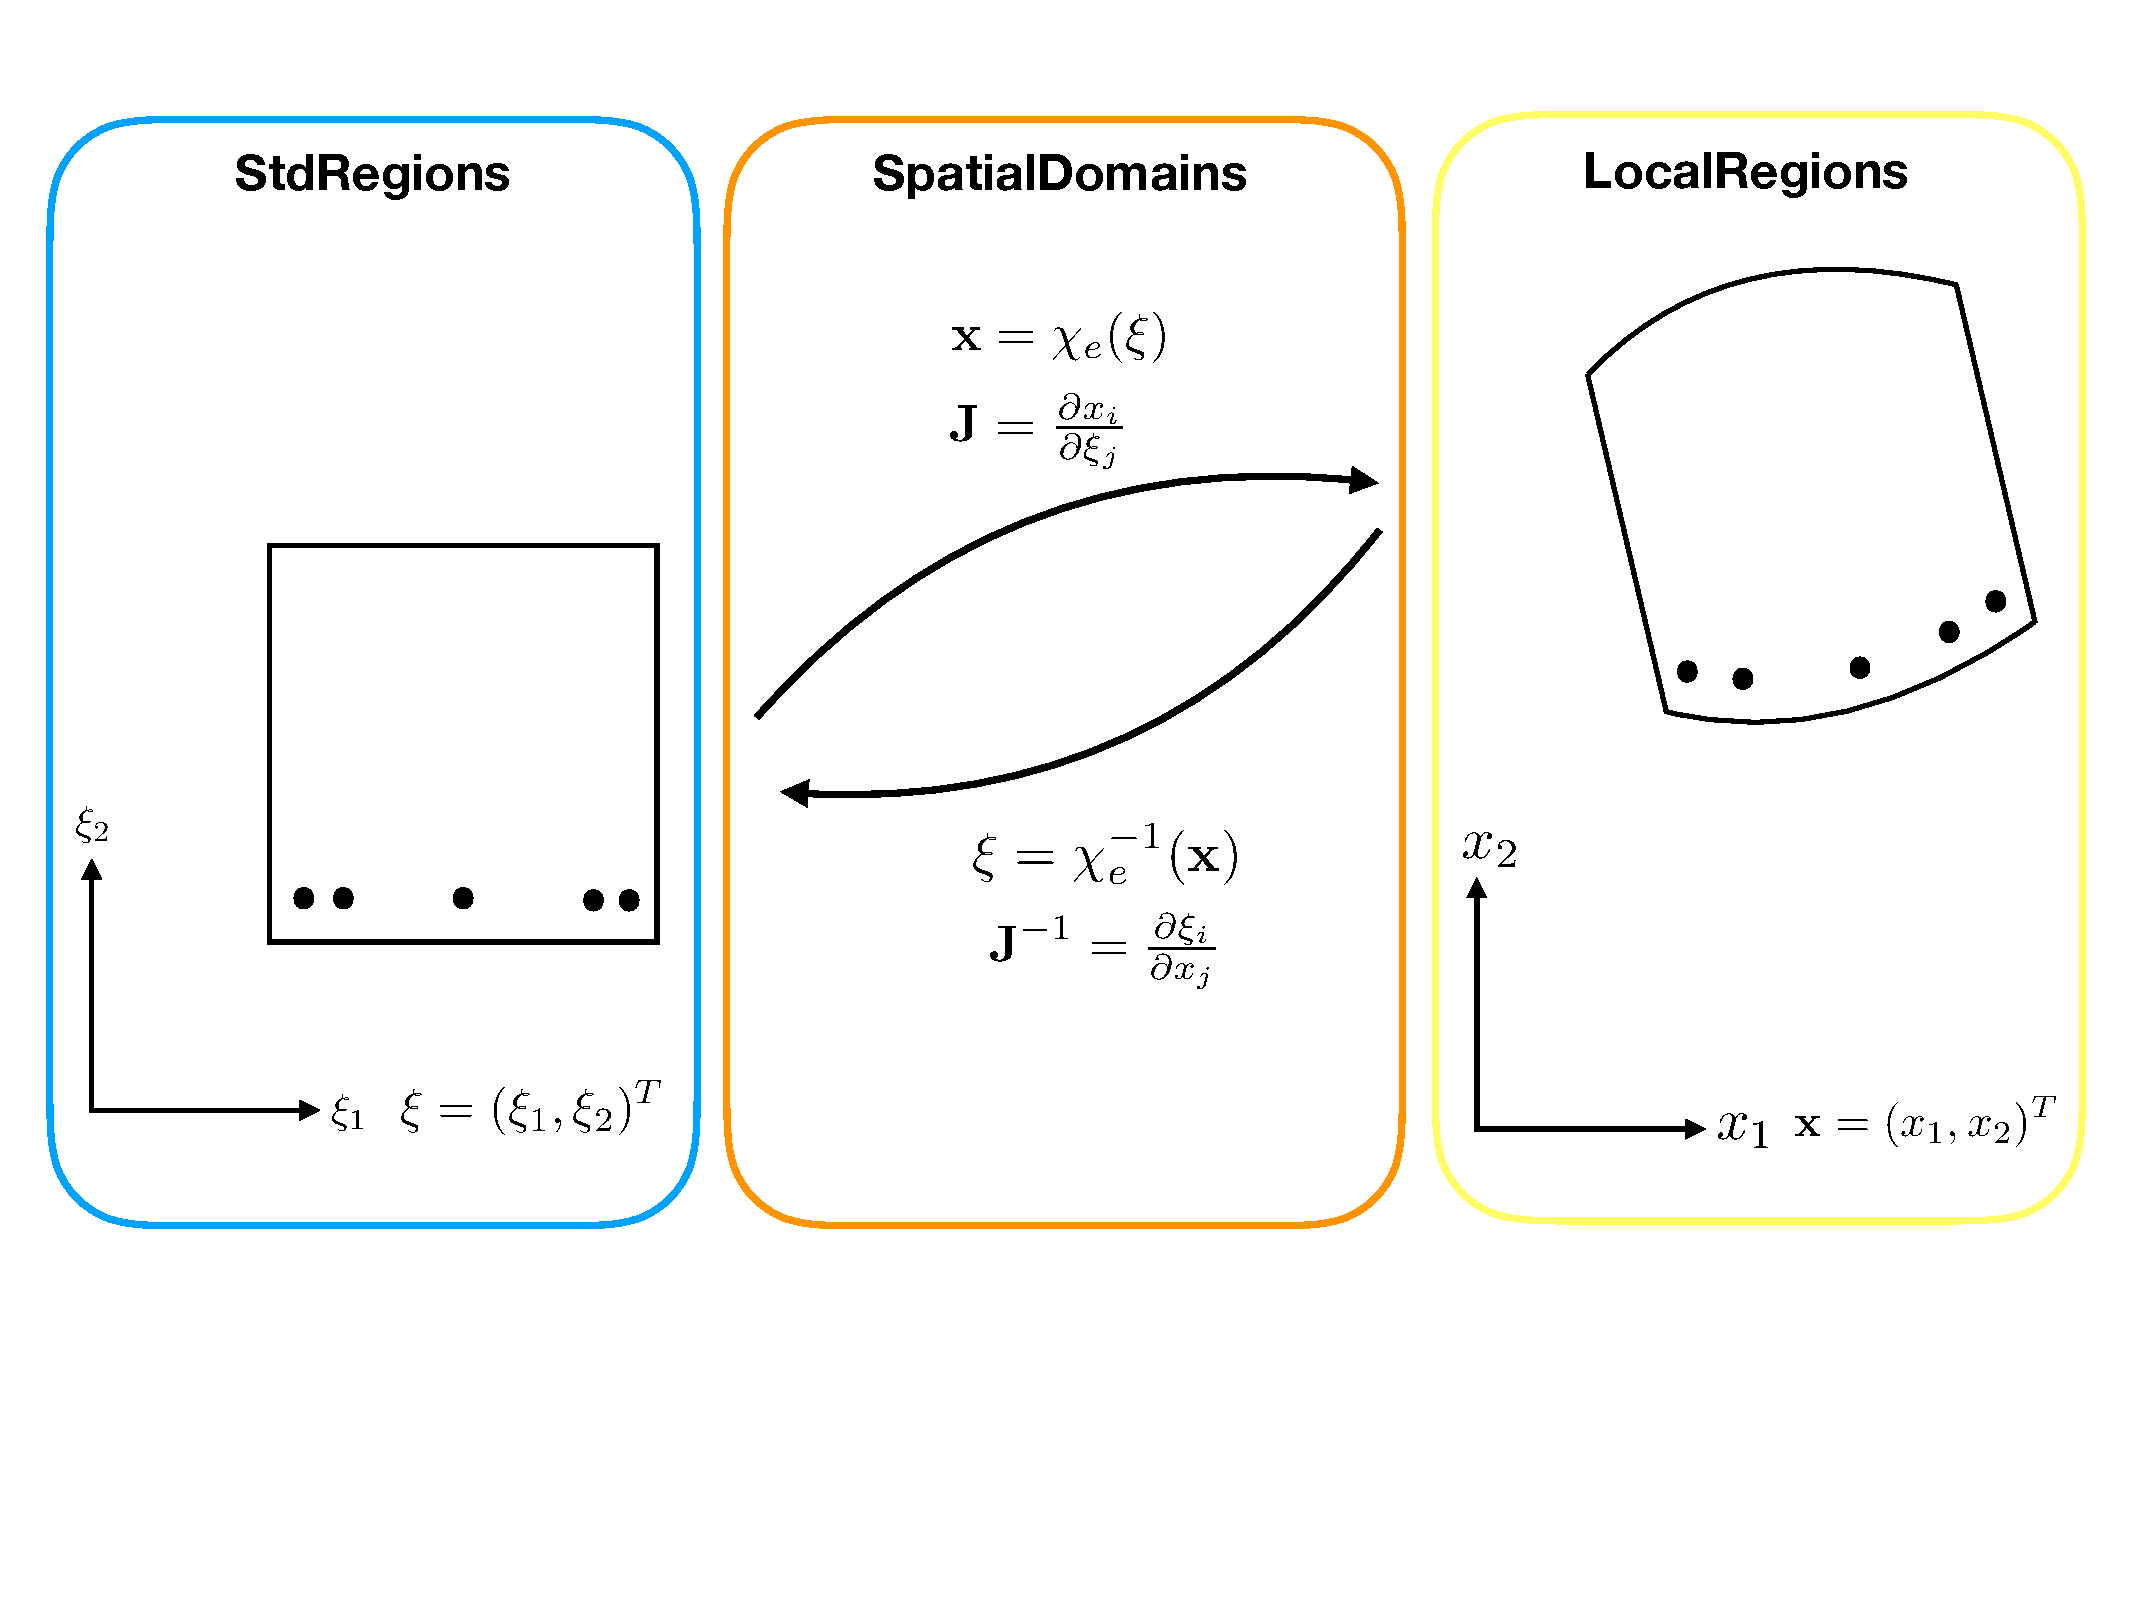
\includegraphics[width=4in]{img/stdtolocal.pdf}
\caption{Diagram showing the LocalRegion (yellow) {\em is-a} StdRegion (blue) which {\em has-a} SpatialDomain (orange) in terms of coordinate systems and mapping functions. This diagram highlights how points (positions in space) are mapped between different (geometric) regions.}
\label{intro:stdtolocal}
\end{figure}

Since $\Psi$ lives on $E_S = [-1,1] \times [-1,1]$ (i.e. $\Psi:E_S\rightarrow\mathbb{R}$) and is for this example polynomial, we can integrate it exactly (to machine precision) using Gaussian integration, and we can differentiate it by writing it in a Lagrange basis and forming a differential operator matrix to act on values of the function evaluated at points.   If the function were not polynomial but instead only a smooth function, we could approximate it with quadrature and decide an appropriate basis by which to 
approximate its derivatives.  All the routines needed for differentiating and integrating polynomials over various standard regions are contained within the StdRegions 
directory (and will be discussed in Chapter \ref{chap:stdregions}).   A local region expansion, such as a basis defined on a quadrilateral element, QuadExp, is a linear combination of basis functions over its corresponding standard region as mapped by
information contained within its spatial domain mapping.  Local region class definitions are in the LocalRegions directory (and will be discussed in Chapter \ref{chap:localregions}).  Using the inheritance language of C++, we would say that a local region {\em is-a} standard region and
{\em has-a} spatial domain object.  The SpatialDomains directory contains information that expresses the mapping function $\chi(\cdot)$ from the standard region
to a local region.  SpatialDomains is explored in Chapter \ref{chap:spatialdomains}.  In the case of our quad example, the SpatialDomain object held by a QuadExp would connect the local region to its StdRegion parent,
and correspondingly would allow integration and differentiation in world space (i.e., the natural coordinates in which the local expansion lives).  If $E$ denotes our
geometric region in world space and if $F:E\rightarrow\mathbb{R}$ is built upon polynomials over its standard region, then we obtain $F(x_1,x_2) = \Psi(\chi^{-1}(x_1,x_2))$.  Note that even though $\Psi$ is polynomial and $\chi$ is polynomial, the composition using the inverse of $\chi$ is not guaranteed to be polynomial: it is only
guaranteed to be a smooth function. 

Putting this in the context of MultiRegions, we arrive at Figure \ref{intro:structure1}.  The MultiRegions directory (which will be discussed in Chapter \ref{chap:multiregions}) contains various data structures that combine
local regions.  One can think of a multi-region as being a set of local region objects in which some collection of geometric and/or function properties are enforced.
Conceptually, one can have a set of local region objects that have no relationship to each other in space.   This is a set in the mathematical sense, but not really
meaningful to us for solving approximation properties.  Most often we want to think of sets of local regions as being collections of elements that are geometrically
contiguous -- that is, given any two elements in the set, we expect that there exists a path that allows us to trace from one element to the next.   Assuming
a geometrically continuous collection of elements, we can now ask if the functions built over those elements form a piece-wise discontinuous approximation
of a function over our multiregion or a piece-wise continuous $C^0$ approximation of a function over our multiregion.

\begin{figure}[htb]
\centering
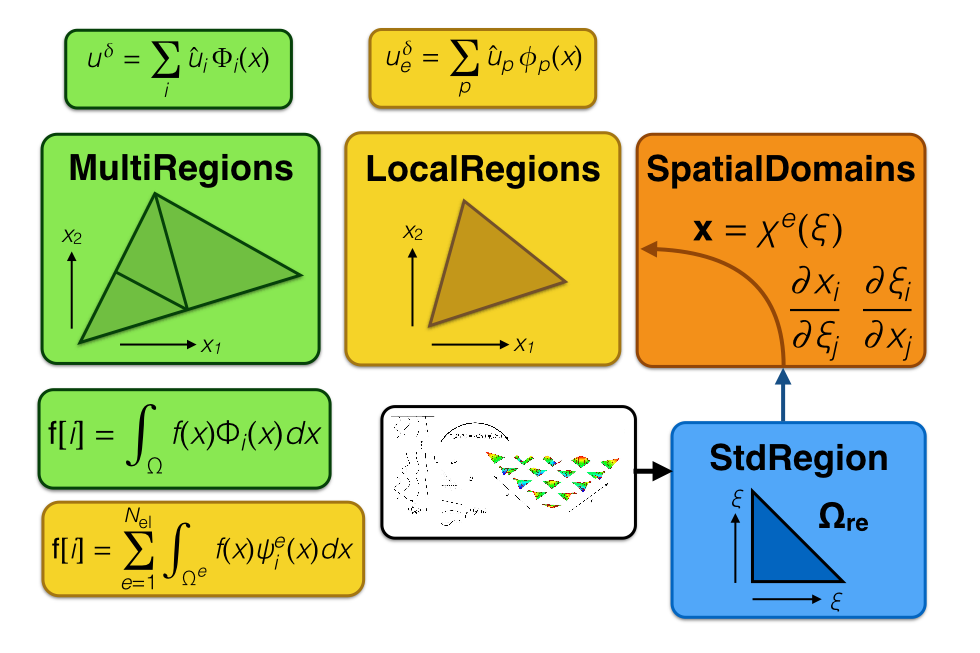
\includegraphics[width=4in]{img/structure1.png}
\caption{Diagram showing how a MultiRegion (green) contains a collection of LocalRegions (yellow), where a LocalRegion {\em is-a} StdRegion (blue) which {\em has-a} SpatialDomain (orange) in terms of coordinate systems and mapping functions.  This diagram highlights the expansions of the solution formed over each geometric domain.}
\label{intro:structure1}
\end{figure}


%%%%%%%%%%%%%%%%%%%%%%%%%%%%%%
\subsubsection{Top-Down Perspective}

The top-down perspective on the library is best understood from Figure \ref{intro:structure2}.  From this perspective, we are interested in understanding 
{\nek} from the solvers various people have contributed.  

\begin{figure}[htb]
\centering
\includegraphics[width=4in]{img/structure2.png}
\caption{Diagram showing the top-down perspective on library components.  Various solvers (along the top) can capitalize on generic SolverUtils and are built upon
the core {\nek} libraries consisting of MultiRegions (green), Collections (red), LocalRegions (yellow), SpatialDomains (orange) and StdRegions (blue).  The most 
generic mathematical and computer science features are contained within LibUtilities, which in part draws from various community resources such as Boost, Metis, etc.}
\label{intro:structure2}
\end{figure}


\section{Assumed Proficiencies}

This developer's guide is designed for the experienced \shp{} user who wishes to go beyond
using various \nek{} solvers and possibly to add new features or capabilities at the library,
solver or utilities levels.  Since the focus of this document is \nek{}, we cannot 
recapitulate all relevant mathematical or computer science concepts upon which our
framework is built.  In this section we provide a listing of areas and/or topics of 
assumed knowledge, and we provide a non-exhaustive list of references to help
the reader see the general areas of additional reading they may need to benefit fully
from this manual.

We assume the reader has a familiarity and comfort-level with the following areas:

\begin{enumerate}
\item Finite Element Methods (FEM) ~\cite{Hughes87,Schwab,BaSzKa81} and more generally the mathematical ideas 
surrounding continuous Galerkin (cG) methods.  This includes basic calculus of variation concepts, basic
partial differential equation knowledge, and general forms of discretization and approximation.

\item Polynomial Methods~\cite{CanutoHQZ87,Funaro92,HGG}, and in particular concepts surrounding polynomial
spaces, basis functions and numerical differentiation and quadrature.

\item Spectral Element Methods (SEM)~\cite{DevilleFM02,KaSh05}.

\item Discontinuous Galerkin Methods \cite{CockburnKS,HesthavenW08}.

\item Scientific Computing~\cite{Heath,KarniadakisK03}.  We assume a graduate-level proficiency in basic
computational techniques such as dealing with numerical precision (accuracy and conditioning), root-finding algorithms,
differentiation and integration, and basic optimization.

\item Linear Algebra \cite{TrefethenB97,Demmel97}.  We assume a strong knowledge of linear algebra and a reasonable 
comfort level with the various numerical algorithms used for the solution of symmetric and non-symmetric linear systems.
\end{enumerate}

\section{Other Software Implementations and Frameworks}

In the last ten years a collection of software frameworks has been put forward to try to bridge the gap between the 
mathematics of high-order methods and their implementation. 
A number of software packages already exist for fluid dynamics which implement
high-order finite element methods, although these packages are typically targeted at a specific
domain or provide limited high-order capabilities as an extension.
A major challenge many practitioners have with
spectral/{\em hp\/} elements and high-order methods, in general, is the complexity (in terms of algorithmic design) they
encounter. In this section, we give an incomplete but
representative summary of several of these attempts to overcome this challenge.

The \emph{Nektar flow solver} is the predecessor to \nek{} and
implements the \shp{} element method for solving the incompressible
and compressible Navier-Stokes equations in both 2D and 3D. While it is widely
used and the implementation is computationally efficient on small parallel problems,
achieving scaling on large HPC clusters is challenging. Semtex \cite{BlSh04}
implements the 2D spectral element method coupled with a Fourier expansion in
the third direction. The implementation is highly efficient, but can only be
parallelised through Fourier-mode decomposition.
Nek5000 \cite{Nek5000} is a 3D spectral element code, based on hexahedral
elements, which has been used for massively parallel simulations up to 300,000
cores. The Non-hydrostatic Unified Model of the Atmosphere (NUMA) \cite{GiraldoKC13} is a spectral element framework that employs continuous 
and discontinuous Galerkin
strategies for solving a particular problem of interest, but in a way on which others could adopt and build.  
Hermes \cite{VeSoZi07} implements hp-FEM for two-dimensional problems and
has been used in a number of application areas. Limited high-order finite
element capabilities are also included in a number of general purpose PDE
frameworks including the DUNE project \cite{DeKlNoOh11} and deal.II
\cite{BaHaKa07}.
% %
FEniCS \cite{FEniCS} is a collaborative project for the development of scientific computing tools, with a particular focus 
on the automated solution of differential equations by finite element methods (FEM).  Through the use of concepts such as meta-programming,
FEniCS tries to keep the solving of PDEs with FEM, from the application programmers' perspective, as close to the mathematical expressions
as possible without sacrificing computational efficiency.
%%
A number of codes also implement high-order finite element methods on
GPGPUs including nudg++, which
implments a nodal discontinuous Galerkin scheme \cite{HeWa07}, and PyFR
\cite{WiFaVi14}, which supports a range of flux reconstruction techniques.

\section{How to Use This Document}

In the next chapter, we will introduce the reader to various computer science tools and ideas upon which we rely heavily in our development and deployment of {\nek}.  The remainder of this developer's guide is then partitioned into three parts.

In Part \ref{part:library}, we provide an overview of the various data structures and algorithms that live within the {\em library} subdirectory.  We think of the library as containing all the basic building blocks of the {\nek} code, as discussed above.  In this part of the developer's guide, we have dedicated a chapter to each subdirectory within the library.  Each chapter contains three main sections.  The first section of a chapter provides an overview of the mathematical concepts and terminology used within the chapter.  This is not meant to be a detailed tutorial, but rather a reminder of basic concepts.  The second section of a chapter provides a detailed description of the data structures introduced in that part of the library.  The third section of a chapter is dedicated to explaining the algorithmic aspects of the library.  Instead of going function by function or method by method, we have decided to structure this section in the style of ``frequently asked questions" (FAQ).  Based upon our long experience with students, postdocs and collaborators, we have distilled down a collection of questions that we will use (from the pedagogical perspective) to allow us to drill down into key algorithmic aspects of the library.

In Part \ref{part:solvers}, we provide an overview of the many solvers implemented on top of the {\nek} library.  Each chapter is dedicated to a different solver, and correspondingly may take on a slightly different style of presentation to match the depth of mathematical, computer science and engineering knowledge to understand the basic data structures and algorithms represented there.

In Part \ref{part:utilities}, we provide an overview of many of the utilities often used in our simulation pipeline -- from things that aid the user in the preprocessing steps such as setting up parameter files and meshing to the postprocessing step of field conversion for visualization.

How you engage with this material is based upon your goals.  If your goal is to:

\begin{itemize}
\item Introduce a new solver, then you would want to jump to Part \ref{part:solvers} and see how other solvers have been built.  Then, depending on what library functions are needed, you may need to step back into the library parts of this manual to understand how to use some of our basic library functionality.
\end{itemize} 








%

\chapter{Preliminaries}


%%%%%%%%%%%%%%%%%%%%%%%%%%%%%%%%%%%%%%%%%%%%%%%%%%
\section{Summary of Development Tools and Best Practices}

%%%%%%%%%%%%%%%%%%%%%%%%%%%%%%%%%%%%%%%%%%%%%%%%%%

\subsection{General Resources}

\subsubsection{Mailing List}

Please make sure that you sign up to the {\nek} mailing list. This can be done at the following URL:

\url{https://mailman.ic.ac.uk/mailman/listinfo/nektar-users}

While the name suggests it is for \textit{users} of Nektar++, this list is also used to ask questions about {\nek} development.

\subsubsection{Blog}

The {\nek} blog (\url{https://www.nektar.info/cat/community})
provides a broad range of posts on topics such as compiling the code
on specific machines, to discussions of {\nek} in specific
application areas, to recently published papers which have made use of
the code.

Contributing to this resource is a valuable way to support the project, as well as promoting your own work.

\subsubsection{Annual Workshop}

In 2015, we held the first {\nek} workshop, which was a great
success and followed by a similar event in 2016. It is now an annual
event and allows first-hand access to the core {\nek} development
team as well as a range of other {\nek} users.

%%%%%%%%%%%%%%%%%%%%%%%%%%%%%%%%%%%%%%%%%%%%%%%%%%

\subsection{Version Control (git)}
\lstset{style=BashInputStyle}

The {\nek} code is managed in a distributed version control system called {\GIT}. To obtain the code directly from the repository and add new content to the repository requires the \texttt{git} command-line tool (or a suitable GUI equivalent). This is available for Linux, Mac OSX and Windows.

If you plan to work with the {\nek} community, you will
need to have a reasonable understanding of the {\GIT}
software.  While it is beyond the scope of this document to discuss
how to use {\GIT}, it is important for someone new to {\GIT} to spend
time understanding how the tool works.  For this purpose, we highly
recommend familiarizing yourself with it using any of the many online
resources (such as \texttt{https://git-scm.com}).

\subsubsection{Anonymous Access}

{\nek} may be cloned anonymously using the following command:

\code{git clone http://gitlab.nektar.info/clone/nektar/nektar.git nektar++}

Your local copy of the code can be updated to include the latest changes in the repository using the command:

\code{git pull}

The \emph{Anonymous Access} approach will provide you with a complete copy of the code, but you will be unable to push changes or new developments back to the repository. For this, you should use \emph{Collaborative Access}.


\subsubsection{Collaborative Access}

Once you are familiar with {\GIT}, have introduced yourself to the
development community (see the mailing list information above), and
are ready to become a contributing developer, you will need to register
an account on the {\nek} Gitlab website:

\url{https://gitlab.nektar.info}.

To use use authenticated access, using your new account, you must first upload the \textbf{public} part of your SSH key to your Gitlab profile. Generating and managing SSH keys is beyond the scope of this document. However, on Linux and OSX, one generally finds these keys in the \lstinline{\$HOME/.ssh} directory.

To upload the key, visit: \url{https://gitlab.nektar.info/profile}, select \emph{SSH keys} from the menu on the left and follow the instructions.

Registering for an account and uploading your SSH key need only be done once.

To clone {\nek}, use the {\GIT} command:

\code{git clone git@gitlab.nektar.info:nektar/nektar.git nektar++}

Note the different URL to use authenticated access, in comparison to the anonymous access.


\subsubsection{Managing and Contributing code}
Code contribution then follows three basic steps:
\begin{enumerate}
    \item Create an \emph{issue} to describe the code updates you are making;
    \item Branch the {\nek} master branch and make your changes on that branch; and 
    \item Submit a merge request on the {\nek} Gitlab website that your updates are ready to be merged into the master branch.
\end{enumerate}

More details regarding the concepts mentioned above is found below. The information is also available in the \texttt{CONTRIBUTING.md} file in the root directory of the code, or online at:
\url{https://gitlab.nektar.info/nektar/nektar/blob/master/CONTRIBUTING.md}

\begin{itemize}
  \item Issues - The initial step for those who wish to add code to the
  master repository is to create an \emph{issue} ticket that describes the
  defect, bug, proposed additions, changes, updates, etc.  This is done on the Gitlab website at:
  
  \url{https://gitlab.nektar.info/nektar/nektar/issues}

  Please ensure you provide sufficient detail when creating the issue to cover
  all of the following (as required): Describe what is being
  requested, why it is important / necessary, an initial list of files
  that may be effected, any potential problems the change/addition may
  cause, and any other information that will help the development team
  understand the request and alert others to your work to avoid duplication of effort.
  
  \item Branches - The second step is to create a {\GIT} branch in which to do
  the actual code development. In your local copy of the {\nek} repository, run the command:
  \begin{lstlisting}  
  git branch <branch-name>
  \end{lstlisting}
  replacing \lstinline{<branch-name>} with a suitable name for your branch. The naming convention used for branches reflects the nature of the change and is composed of a prefix and descriptor, separated by a forward slash. Prefixes are one of:
  \begin{itemize}
      \item \texttt{feature}: used for developments which constitute a new capability in the code;
      \item \texttt{fix}: used for changes to fix a bug in the code;
      \item \texttt{tidy}: used for changes which improve the quality or readability of the code but do not change its function;
      \item \texttt{ticket}: can be used to reference changes which address a specific issue.
  \end{itemize}
  Please choose concise descriptors in all-lowercase, using hyphens to separate words. An example \lstinline{<branch-name>} might therefore be: \lstinline{feature/low-energy-preconditioner}
  
  Now make your new branch active by running the command:
  \begin{lstlisting}
  git checkout <branch-name>
  \end{lstlisting}
  Confirm you are on the correct branch by running:
  \begin{lstlisting}
  git status
  \end{lstlisting}
  which should print something similar to
  \begin{lstlisting}
  On branch <branch-name>
  \end{lstlisting}

  At this point you are all set to make the required modifications to the 
  code in your branch.  As you modify your branch, you can use {\GIT} to
  save and track your changes.

  The following examples show how you can add a file to the list of local
  files that are being tracked, display differences between the current
  file and the original file, and commit the file.  
  \begin{lstlisting}
  git add library/LibUtilities/BasicUtils/my_new_file.cpp
  git diff --cached
  \end{lstlisting}

  Note \lstinline{--cached} is necessary because \lstinline{my\_new\_file.cpp} was staged using
  the \lstinline{git add} command above.  Note, before you add (stage) the
  file, you can just use \lstinline{git diff}.
  
  To actually create the commit from the staged files, run:
  \begin{lstlisting}
  git commit -m "Added X, Y, Z..."
  \end{lstlisting}
  This commits the file to your local repository. The first line of the log message should be a concise summary of the changes. You can use subsequent lines to provide more details if needed. Use \lstinline{git log} to see the list of previous commits and their messages.
  
  These changes are still local to your computer. To push them up to the main {\nek} repository, use the command
  \begin{lstlisting}
  git push origin
  \end{lstlisting}
\end{itemize}

%%%%%%%%%%%%%%%%%%%%%%%%%%%%%%%%%%%%%%%%%%%%%%%%%%
\subsection{Building (CMake)}

{\nek} uses the \emph{CMake} tool to manage the build process for
the three supported operating systems: Linux, Windows, and OSX.  For
detailed instructions on how to use \emph{CMake} to build {\nek},
including a list of required software dependencies and \emph{CMake}
option flags, please refer to the {\nek} User Guide section 1.3.

\subsection{Testing (CTest)}
Before you are ready to have your code merged into the {\nek}
trunk, you should make sure that it passes the built-in test suite -
in addition to any new tests that you have added for your
updates. To run the test suite, on the command line type:
\begin{lstlisting}  
ctest [-j#]
\end{lstlisting}
  
The \lstinline{-j#} optional argument will run \lstinline{#} tests in parallel
taking advantage of multiple cores on your machine.  It is highly
recommended that your use all available cores to minimize the amount
of time spent waiting for the tests to complete. There are currently
several hundred built-in unit tests for {\nek}.

For more information on testing, see ``Software Testing Approaches'' below.

\subsection{Merge Requests (Gitlab)}
The final step in contributing your code to the
Nektar master repository is to submit a merge request to the
development team using the {\nek} gitlab website:
  
\url{https://gitlab.nektar.info/nektar/nektar/merge\_requests}
  
Submitting a merge request will automatically trigger the continuous integration (CI) system, which will build and test your code on a range of platforms. You can monitor the progress of these tests from the merge request page. Selecting individual workers will take you to the buildbot website from which you can examine any failures which have occurred.
  



%%%%%%%%%%%%%%%%%%%%%%%%%%%%%%%%%%%%%%%%%%%%%%%%%%
\section{Core Nektar++ Programming Concepts}
\lstset{style=C++Style}

This section highlights some of the programming features that are used
extensively within {\nek}. While much of the code consists of
standard C++ practices, in some of the core infrastructure there are
several practices that may be only familiar to programmers who have
developed code using more advanced C++ features.  Below we give a
short summary of these entities in order to provide a starting point
when working with these features. We begin with more well known
features and end with some advanced techniques.  Note, it is not the
purpose of the following sections to cover in detail each of these
important concepts, but instead to give a brief overview of them such that the developer may look to other, more in-depth, sources if
they require further guidance.

\subsection{Namespaces}
Many C++ software projects place their code in a namespace so as to avoid conflicts with other code when included in larger applications.  It is important to note that {\nek} uses a hierarchy of namespaces for most of the defined data structures.  The top level namespace is always ``Nektar'', with the second level usually corresponding to the name of the library to which the code belongs. For example:
\begin{lstlisting}
namespace Nektar
{
namespace StdRegions
{
    ...
}
}
\end{lstlisting}

With this in mind, when you see something like \lstinline{Nektar::SpatialDomains::...}, you can usually assume that the second item (in this case \lstinline{SpatialDomains}) is a namespace, and not a class.

\textbf{Note:} To make better use of the 80 character width, generally enforced across the {\nek} source code, we choose not to indent the contents of \lstinline|namespace| blocks.


\subsection{C++ Standard Template Library (STL) }
{\nek} uses of the C++ STL extensively.  This consists of common data structures and algorithms, such as map and vector, as well as many of the extensions once found in the Boost library that have become part of the C++ standard and are now used directly.

One of the most important of these features is
the use of Shared Pointers (\lstinline|std::shared_ptr|).  Most developers are
somewhat familiar with ``smart pointers'' (pointers used to track
memory allocation and to automatically deallocate the memory when it
is no longer being used) for data blocks that are shared by multiple
objects. These smart pointers are used extensively in {\nek} and
one should be familiar with the \lstinline|dynamic_pointer_cast| function
and the concept of the \lstinline|weak_ptr|.  Dynamic casting allows for safely
converting one type of variable into its base type (or vice
versa). For example:
\begin{lstlisting}
std::shared_ptr<FilterCheckpoint> sptr =
        std::dynamic_pointer_cast<FilterCheckpoint>( m_filters[k] );
if( sptr != nullptr ) 
{ 
   // Cast succeeded!
}
\end{lstlisting}

The advantage of using the dynamic cast, in comparison to the C style
cast, is that you can check the return value at run time to verify
that the casting was valid.  A \lstinline|weak_ptr| is a pointer to shared
data with the explicit contract that the weak pointer does not own
the data (and thus will not be responsible for deallocating it).
Weak pointers are used mostly for short-term access to shared data.

Another modern code utility used by {\nek} to support shared
pointers can be seen in {\nek} classes which inherit from
\lstinline|std::enable_shared_from_this|. This allows a class member function to return a shared pointer to itself. Specifically, it makes available the function \lstinline|shared_from_this()| which returns a shard pointer to the object in the given context.

While C++ shared pointers are a powerful resource, there are a
number of intricacies that must be understood and followed when
creating classes and using objects that will be managed by them.
For those not familiar with the C++11 (or previously Boost)
implementation, it is highly recommended that you study them in more
detail then presented here.
  
\subsection{typedefs}
Like most other large codes, {\nek} uses
\lstinline{typedefs} to create short names for new variable types.  You will
see examples of this throughout the code and taking a few minutes to
look at the definitions will help make it easier to follow the code.
In the following example, we create (and explicitly name) the type
\lstinline{ExpansionSharedPtr} to make the code that uses this type easier
to follow. This is particularly true of nested STL data structures where repeated template declarations would make the code harder to follow. A couple of examples are shown below:
\begin{lstlisting}
typedef std::shared_ptr<Expansion> ExpansionSharedPtr;
typedef std::shared_ptr<std::vector<std::pair<GeometrySharedPtr, int>>>
GeometryLinkSharedPtr;
\end{lstlisting}
If you are not familiar with the use of typedefs, you should take
time to read about them (there are many short summaries
available on the web).

\subsection{Forward Declarations}
There are two ways that an existing class
type can be specified when declaring a new class in a header file.  The
existing class can either be declared in name only, or declared in its entirety, before being used. In the latter case, one typically includes the header file declaring the full class. If the new class declaration only references the existing class in the form of a pointer or reference then the entire class declaration is not needed and the compiler only needs an assurance that the class exists. For this case, we can use a \emph{forward declaration} which tells the compiler the name of the existing class. 
However, if functions of the existing class are called (within the new header file) or the class is used by value, then the full declaration is needed.

Forward declaring a class is achieved as shown in the following example:
\begin{lstlisting}
class LinearSystem;
\end{lstlisting}
This statement tells the compiler the class \lstinline{LinearSystem} exists and, as long as we only make reference to it as a pointer (\lstinline{LinearSystem* l}) or by reference (\lstinline{const LinearSystem & l}), then the compiler does not require any further information.

An advantage to using forward declarations where possible is that the header file does not need to \lstinline{#include} the entire existing class and any header files referenced within.  This allows for a
cleaner header files and faster compilation as the compiler can process (often significantly) fewer lines of code.

\textbf{Note}: The full class declaration is most likely needed in the new class implementation file (.cpp) as reference to the existing class's members will presumably be made.
  
\subsection{Templated Classes and Specialization}
Most C++ developers are
familiar with basic class templating.  However, many have not needed
to use explicit template specialization.  This is the process of
implementing customised behaviour for one or more of the specific instances of a template when
the compiler will not be able to instantiate a generic version for
the class, or when different code is needed based on different
versions of the class.  For example:
\begin{lstlisting}
  template<typename Dim, typename DataType> 
  class Array;
  
  template<typename DataType>
  class Array<OneD, const DataType> {
    // Explicit coding of class methods and variables specific to
    // this version of Array are found here.
  };
\end{lstlisting}

In the above example, on the first line the generic templated
\lstinline{Array} class is declared. There are two template parameters: the dimension and the element type. The second line shows an explicit
template specialisation of the \lstinline{Array} class for a one-dimensional (version of) \lstinline{Array}.  When explicitly specialising a class, the programmer
will write code that is specific to the datatype used in specifying
the class.  This includes explicitly writing code for one, some, or
all of the methods of the class.

It is important to understand template specialization when dealing
with the {\nek} core libraries so that the developer can
determine which (specialized version of the) class is being used,
and to know that when updating classes with varied specializations,
that it may be required to update code in several places (ie, for
each of the specializations).

\subsection{Multiple Inheritance and the \lstinline{virtual} Keyword}
When diving into many {\nek} classes, you will see the use of multiple
inheritance (where a class inherits from more than one parent
class).  When the parent class does not inherit from other classes,
then the inheritance is straightforward and should not cause any
confusion.  However, when a class has grandparents, many times that
grandparent class is the same class but is inherited through multiple
parents.  To account for this, class inheritance should use the
\lstinline{virtual} keyword.  This specifies that if a class has multiple
grandparents (that happen to be the same class), that only one copy of
the grandparent class members should actually be instantiated. For example:
\begin{lstlisting}
class Expansion2D : virtual public Expansion,
                    virtual public StdRegions::StdExpansion2D
{...}
\end{lstlisting}


\subsection{Virtual Functions and Inheritance}
Within {\nek}, classes
that inherit from a parent class and override one of the parent
class methods, use the concept of virtual functions. The function is prefixed with a \lstinline{v_}, such as \lstinline{v_Function()}, as a naming convention.  This is a visual reminder that the function overrides a parent class function. For example:
\begin{lstlisting}
NekDouble TriExp::v_Integral(const Array<OneD, const NekDouble> &inarray)}
\end{lstlisting}

\subsection{Const keyword}
While the \lstinline{const} keyword is known to most C++
developers, it is used (as it should be) liberally in {\nek} for functions,
function parameters, returning pointers to class data, and variable
constants within functions.  It is easy to neglect using \emph{const}
to mark all cases where a variable should be considered constant.
However, its use can substantially reduce accidental errors and
allow for accelerated debugging. The \lstinline{const} qualifier should be used wherever a variable does not change including 1) parameters passed to
functions, 2) variables in functions (or classes) that do not change
value during their lifetime, 3) on the return type of functions that return pointers to data that should not be changed, and 4) on methods that do not
change data within the class. The compiler will then produce an error if we (accidentally) attempt to make a change which violates a \lstinline{const}.

\subsection{Function pointers and bind}
Function pointers
  (\lstinline{std::function}) are similar to pointers to data, except that
  they point to functions - and thus allow a function to be invoked
  indirectly (in other words, without explicitly writing the function
  call (name) directly in code).  This technique is used by {\nek}
  in a number of places, with \lstinline{NekManager} being a prime example.
  The \lstinline{NekManager} class is used to create objects of a specific
  type during the execution of the program.  When a \lstinline{NekManager} is
  created (constructed), it is provided with a pointer to a function
  that will (later) be called to generate the objects to be managed when required.  While
  the \emph{creation} function that is provided to the \lstinline{NekManager}
  takes a number of parameters, in many cases some of the values to
  those parameters will be fixed.  To handle this situation, {\nek}
  uses the \lstinline{std::bind( f )} function, which creates a new function
  based on supplied original function \lstinline{f}, but specifies that one
  or more parameters of \lstinline{f} are fixed at the time that \lstinline{f} is created and only those bound parameter values will be used when
  \lstinline{f} is later invoked.  


\subsection{Memory Pools and NekArray}
An Array is a thin wrapper around native arrays. Arrays provide all the
functionality of native arrays, with the additional benefits of automatic use of
the Nektar++ memory pool, automatic memory allocation and deallocation, bounds
checking in debug mode, and easier to use multi-dimensional arrays.

Arrays are templated to allow compile-time customization of its dimensionality
and data type.

Parameters:
\begin{itemize}
    \item \lstinline{Dim} Must be a type with a static unsigned integer called
    \lstinline{Value} that specifies the array's dimensionality. For example
    \begin{lstlisting}
    struct TenD {
        static unsigned int Value = 10;
    };
    \end{lstlisting}
    \item \lstinline{DataType} The type of data to store in the array.
\end{itemize}

It is often useful to create a class member Array that is shared with users of
the object without letting the users modify the array. To allow this behavior,
\lstinline{Array<Dim, DataType>} inherits from 
\lstinline{Array<Dim, const DataType>}. The following
example shows what is possible using this approach:
\begin{lstlisting}
class Sample {
public:
    Array<OneD, const double>& getData() const { return m_data; }
    void getData(Array<OneD, const double>& out) const { out = m_data; }

private:
    Array<OneD, double> m_data;
};
\end{lstlisting}
In this example, each instance of Sample contains an array. The getData
method gives the user access to the array values, but does not allow
modification of those values.



%%%%%%%%%%%%%%%%%%%%%%%%%%%%%%%%%%%%%%%%%%%%%%%%%%
\section{Design Patterns}
\subsection{Template pattern}
\label{s:template-pattern}
The template pattern is used frequently within {\nek} to provide a common interface to a range of related classes. The base class declares common functionality or algorithms, in the form of public functions, deferring to protected virtual functions where a specific implementation is required for each derived class. This ensures code external to the class hierarchy sees a common interface.

In the top level parent class you will find the interface functions, such as
\lstinline{Function()}, declared as public members. In some cases, these may implement a generic algorithm common to all classes. In the limit that the function is entirely dependent on the derived class, it may call through to a virtual counterpart, usually named \lstinline{v_Function()}. These functions are usually protected to allow them to be called directly by other classes in the inheritance hierarchy, without exposing them to external classes.

As an example of this, let us consider a triangle
element (\lstinline{TriExp}).  The \lstinline{TriExp} class (eventually) inherits from the \lstinline{StdExpansion} class.  The \lstinline{StdExpansion} defines the \lstinline{Integral()} function which is used to provide integration over an element.  However, in this case, the implementation is shape-specific. Therefore \lstinline{StdExpansion::Integral()} calls the (in this case) \lstinline{TriExp::v_Integral()} function.  We should also note that while \lstinline{TriExp::v_Integral()} does setup work, it then makes use of its parent's \lstinline{StdExpansion2D::v_Integral()} function to calculate the final value. This is only possible if the \lstinline{v_Integral()} function was declared as protected.

\subsection{Abstract Factory Pattern}

{\nek} makes extensive use of the \emph{Factory Pattern}.
Factories are used to create (allocate) instances of classes using class-specific creator functions. More
specifically, a factory will create a new object of some
sub-class type but return a base class pointer to the new
object. In general, there are two ways that a factory knows what
specific type of object to generate: 1) The Factory's build
function (\lstinline{CreateInstance()}) is
passed a key that details what to build; or 2) The factory may
have some intrinsic knowledge detailing what objects to create. The first case is almost exclusively used throughout {\nek}.
The factory pattern provides the following benefits:
\begin{itemize}
\item Encourages modularisation of code such that conceptually related
algorithms are grouped together;
\item Structuring of code such that different implementations of the same
concept are encapsulated and share a common interface;
\item Users of a factory-instantiated modules need only be concerned with the
 interface and not the details of underlying implementations;
\item Simplifies debugging since code relating to a specific implementation
 resides in a single class;
\item The code is naturally decoupled to reduce header-file dependencies and
 improves compile times;
\item Enables implementations (e.g. relating to third-party libraries) to be
 disabled through the build process (CMake) by not compiling a specific 
 implementation, rather than scattering preprocessing statements throughout the
 code.
\end{itemize}


\subsubsection{Implementing the factory pattern}
The \lstinline{NekFactory} class implements the factory pattern in Nektar++.
There are two distinct aspects to creating a factory-instantiated collection of
classes: defining the public interface, and; registering specific
implementations. Both of these tasks involve adding mostly standard boilerplate code.

It is assumed that we are writing a code which implements a particular \emph{concept} or
\emph{capability} within the code, for which there are (potentially) multiple implementations. The
reasons for multiple implementations may be low level, such as alternative
algorithms for solving a linear system, or high level, such as selecting from a
range of PDEs to solve. The \lstinline{NekFactory} can be used in both cases and applied in exactly the same way.

\subsubsection{Creating a concept (base class)}
A base class must be defined which prescribes an implementation-independent
interface. In Nektar++, the template method pattern (see Section~\ref{s:template-pattern} above) is used, requiring public
interface functions to be defined which call through to protected virtual implementation methods. This is because the factory returns the newly created object via a base-class pointer and the objects will almost always be used via this base class pointer. Without a public interface in the base class, much of the benefits and generalisation of code offered by the factory pattern would be lost.
The virtual functions will be overridden in the specific implementation classes.
In the base class these virtual methods should normally be defined as pure virtual, since there is typically no implementation and we will never be explicitly instantiating this base class.

As an example we will create a factory for instantiating different
implementations of some concept \inlsh{MyConcept}, defined in
\inlsh{MyConcept.h} and \inlsh{MyConcept.cpp}.

First in \inlsh{MyConcept.h}, we need to include the NekFactory header
\begin{lstlisting}
#include <LibUtilities/BasicUtils/NekFactory.hpp>
\end{lstlisting}

The following code should then be included just before the base class
declaration (within the same namespace as the class):
\begin{lstlisting}
class MyConcept

// Datatype for the MyConcept factory
typedef LibUtilities::NekFactory< std::string, MyConcept, 
            ParamType1,
            ParamType2 > MyConceptFactory;
MyConceptFactory& GetMyConceptFactory();
\end{lstlisting}

The template parameters to the \lstinline{NekFactory} define the datatype of the key used to retrieve a
particular implementation (usually a string, enum or custom class such as
\lstinline{MyConceptKey}), the base class datatype (in our case \lstinline{MyConcept} and a list
of zero or more parameters which are taken by the constructors of all
implementations of the type \lstinline{MyConcept} (in our case we have two). Note
that all implementations must take the same parameter list in their constructors. Since we have not yet declared the base class type \lstinline{MyConcept}, we have forward-declared it above the \lstinline{NekFactory} type definition.

The normal definition of our base class then follows:
\begin{lstlisting}
class MyConcept 
{
    public:
        MyConcept(ParamType1 p1, ParamType2 p2);
        ...
};
\end{lstlisting}

We must also define a shared pointer for our base class, which should be declared outside the base class declaration.
\begin{lstlisting}
typedef boost::shared_ptr<MyConcept> MyConceptShPtr;
\end{lstlisting}


\subsubsection{Creating a specific implementation (derived class)}
A new class, derived from the base class above, is defined for each specific implementations of a concept. It is these
specific implementations which are instantiated by the factory.

In our example we will have an implementations called \lstinline{MyConceptImpl1}
defined in \inlsh{MyConceptImpl1.h} and \inlsh{MyConceptImpl1.cpp}. In the
header file we include the base class header file
\begin{lstlisting}
#include <MyConcept.h>
\end{lstlisting}

We then define the derived class as one would normally:
\begin{lstlisting}
class MyConceptImpl1 : public MyConcept
{
...
};
\end{lstlisting}

In order for the factory to work, it must know two things:
\begin{itemize}
\item that \lstinline{MyConceptImpl1} exists; and
\item how to create an instance of it.
\end{itemize}

To allow the factory to create instances of our class we define a \emph{creator} function in our class, which may have arbitrary name, but is usually called \lstinline{create} out of convention:
\begin{lstlisting}
/// Creates an instance of this class
static MyConceptSharedPtr create(
            ParamType1 p1,
            ParamType2 p2)
{
    return MemoryManager<MyConceptImpl1>::AllocateSharedPtr(p1, p2);
}
\end{lstlisting}
The example above the \lstinline{create} function simply creates an instance of \inlsh{MyConceptImpl1} using the {\nek} memory manager and the
supplied parameters. It must be a \lstinline{static} function because we are not operating on any existing instance and it should return a shared pointer to a base class object (rather than a \lstinline{MyConceptImpl1} shared pointer), since the point of the factory is that the calling code does not know about specific implementations. An advantage of having each class providing a creator function is that it allows for \emph{two-stage initialisation} -- for example, initialising base-class variables based on the derived type.

The final task is to register each of our implementations with the factory. This is done 
using the \lstinline{RegisterCreatorFunction} member function of the \lstinline{NekFactory}.
However, we wish this to happen as early on as possible (so we can use the 
factory straight away) and without needing to explicitly call the function for 
every implementation at the beginning of our program (since this would again 
defeat the point of a factory)! One solution is to use the function to 
initialise a static variable: it will force the function to be executed prior to the start of the \lstinline{main()} routine, and can be located within the class it is registering, satisfying our code decoupling requirements.

In \inlsh{MyConceptImpl1.h} we define a static class member variable with the same datatype as the key used in our factory (in our case \lstinline{std::string}) 
\begin{lstlisting}
static std::string className;
\end{lstlisting}
The above variable can be private since it is typically never actually
used within the code. We then initialise it in \inlsh{MyConceptImpl1.cpp}
\begin{lstlisting}
string MyConceptImpl1::className
        = GetMyConceptFactory().RegisterCreatorFunction(
                                "Impl1", 
                                MyConceptImpl1::create, 
                                "First implementation of my concept.");
\end{lstlisting}
The first parameter specifies the value of the key which should be used to
select this implementation. The second parameter is a function pointer to the
static function which should be used by the factory to instantiate our class. The third parameter provides a description which can be printed when listing the available \lstinline{MyConcept} implementations. A specific implementation can be registered with the factory multiple times if there are multiple keys which should instantiate an object of this class.


\subsubsection{Instantiating classes}
To create instances of MyConcept implementations elsewhere in the code, we must
first include the ''base class'' header file
\begin{lstlisting}
#include <MyConcept.h>
\end{lstlisting}
Note we do not include the header files for the specific MyConcept 
implementations anywhere in the code (apart from \inlsh{MyConceptImpl1.cpp}).
If we modify the implementation, only the implementation itself requires 
recompilation and the executable relinking.

We create an instance by retrieving the \lstinline{MyConceptFactory} and calling the \lstinline{CreateInstance} member function of the factory, for example,
\begin{lstlisting}
ParamType p1 = ...;
ParamType p2 = ...;
MyConceptShPtr p = GetMyConceptFactory().CreateInstance( "Impl1", p1, p2 );
\end{lstlisting}

Note that the instance of the specific implementation is used through the pointer \lstinline{p}, which is of type \lstinline{MyConceptShPtr}, allowing the use of any of the public interface functions in the base class (and therefore the specific implementations behind them) to be
called, but not directly any functions declared solely in a specific
implementation.



%%%%%%%%%%%%%%%%%%%%%%%%%%%%%%%%%%%%%%%%%%%%%%%%%%
\section{Software Testing Approaches}

%%%%%%%%%%%%%%%%%%%%%%%%%%%%%%%%%%%%%%%%%%%%%%%%%%
\subsection{Unit Tests}

Unit testing, sometimes called ``module testing'' or ``element testing'', is a
software testing method by which individual ``units'' of source code
are tested to determine whether they are fit for use
\cite{KFN-testing}.  Unit tests are added to {\nek} through the
CMake system, and implemented using the Boost test framework.
As an example, the set of linear algebra unit tests is
listed in this file:

\inlsh{.../library/UnitTests/LibUtilities/LinearAlgebra/CMakeLists.txt}

and the actual tests are implemented in this file:

\inlsh{.../library/UnitTests/LibUtilities/LinearAlgebra/TestBandedMatrixOperations.cpp}

To register a new test, you use \lstinline{BOOST_AUTO_TEST_CASE( TestName )},
implement the unit test, and test the result using
\lstinline{BOOST_CHECK_CLOSE(...)}, \lstinline{BOOST_CHECK_EQUAL(...)}, etc. Unit
tests are invaluable in maintaining the integrity of the code base and
for localizing, finding, and debugging errors entered into the code. It is
important to remember a unit test should test very specific
functionality of the code - in the best case, a single function should be
tested per unit test.

While it is beyond the scope of this document to go into more detail
on writing unit tests, a good summary of the Boost test system can be
found here:

\url{http://www.boost.org/doc/libs/1\_63\_0/libs/test/doc/html/}.


%%%%%%%%%%%%%%%%%%%%%%%%%%%%%%%%%%%%%%%%%%%%%%%%%%
\subsection{Integration, System and Regression Tests}
Integration testing involves testing ecosystems of components and their interoperability. System testing tests complete applications and regression testing focuses on ensuring previously fixed bugs do not resurface. In {\nek} all of these are often colloquially referred to as {\em regression testing}. It is not \emph{white-box} in that it does not examine how the
code arrives at a particular answer, but rather in a \emph{black-box}
fashion tests to see if code when operating on certain data yields the
predicted response \cite{KFN-testing}.

\subsection{Continuous Integration}
{\nek} uses the \emph{buildbot} continuous integration to perform testing of the code across multiple operating systems.  Builds are automatically instigated when merge requests are opened and subsequently when the associated branches receive additional commits.

For more information, go to:

\url{http://buildbot.nektar.info}


%%%%%%%%%%%%%%%%%%%%%%%%%%%%%%%%%%%%%%%%%%%%%%%%%%
%\input{prelims/coding-standard.tex}

%%%%%%%%%%%%%%%%%%%%%%%%%%%%%%%%%%%%%%%%%%%%%%%%%%


%

\part{Building-Blocks of Our Framework (Inside the Library)} \label{part:library}


\import{library/}{library-master}
%%
\part{Solvers} \label{part:solvers}

\import{solvers/}{solvers-master}

%%
\part{Utilities} \label{part:utilities}

\import{utilities/}{utilities-master}

\part{NekPy: Python interface to \nek{}} \label{part:nekpy}

\import{python/}{python-master}


\bibliographystyle{plain}
\bibliography{developers-guide} 

\printindex

\end{document}
